\documentclass{article}
\usepackage[utf8]{inputenc}
\usepackage{authblk}
\usepackage[utf8]{inputenc}
\usepackage{authblk}
\usepackage{amsmath}
\usepackage{mathtools}
\usepackage{wrapfig}
\usepackage{float}
\usepackage{graphicx}
\usepackage{subcaption}
\usepackage[dutch]{babel}
\usepackage{natbib}


\title{Modelleren, maken en meten Verslag 2, Groep B}
\author{De Wispelaere Tobias, Fordeyn Tibo, Decavele Julie, , Dobbelaer Xander \\ Onder leiding van prof. Vincent Bracke, Maarten de Mildt}
\date{}
% \def \id{01702577}
% \def \groep{I}
% \def \opsteling{A}

\usepackage{natbib}
\usepackage{graphicx}

\setlength\paperwidth{20.999cm}\setlength\paperheight{29.699cm}\setlength\voffset{-1in}\setlength\hoffset{-1in}\setlength\topmargin{1.499cm}\setlength\headheight{12pt}\setlength\headsep{0cm}\setlength\footskip{1.131cm}\setlength\textheight{25cm}\setlength\oddsidemargin{2.499cm}\setlength\textwidth{15.999cm}

\makeatletter
    \renewcommand{\maketitle}{
    \begin{center}
    \begin{minipage}{0.15\linewidth}%
    
\includegraphics[width=0.90\linewidth]{~/school/eerste-jaar/eerste-semester/project-MMM/verslag/figures/ugent-logo.png}
    \end{minipage}\hspace{10pt}
    \begin{minipage}{0.8\linewidth}%
    \begin{center}
            \vspace{.35cm}
            {\bf {\Huge \@title}}\\
            \vspace{.2cm}
            \textbf{ \Large \@author}  \\
            \vspace{.15cm}
            \@date \\
            \vspace{.1cm}
    \end{center}
    \end{minipage}%
    \end{center}
    \begin{center}
        % Opstelling: \opsteling \hspace{\fill} \@date \hspace{\fill} Groep:{\bf \space \groep}
    \end{center}
\hrule width \hsize height 2pt \kern 1mm  \hrule width \hsize height 1pt
}
\makeatother

\begin{document}

\maketitle

\section{Sample rates}
De onderstaande tabel bevat de verschillende metingen voor elk van de rates, uitgedrukt in metingen per minuut. Ze zijn geordend volgens snelheid.\\
\\
\begin{tabular}{ |p{3cm}||p{4cm}|p{3cm}|p{3cm}|  }
 \hline
 \multicolumn{2}{|c|}{Tabel 1: Lijst met metingen per minuut van sample rates} \\
 \hline
 Sample rates&Metingen per minuut \\
 \hline
 Normal   & 300   \\
 UI&   1000  \\
 Game &3000 \\
 Fastest    &6000 \\
 \hline
\end{tabular}

\begin{wrapfigure}{r}{5.5cm}
    \label{wrap-fig:1}
    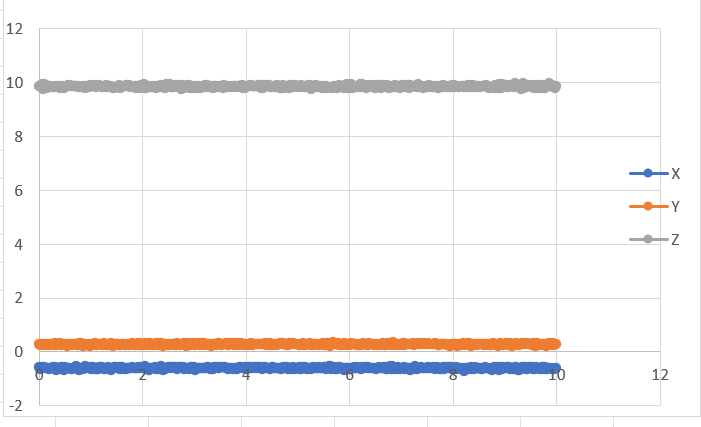
\includegraphics[width=5.5cm]{figures/andereAfb/waardenSchermBoven.png}
    \caption{Grafische voorstelling van de meting met het scherm naar omhoog}
\end{wrapfigure}
\section{Ondervonden valversnelling in rust}
Op de grafiek zien we de tijd in seconden op de X-as, en de valversnelling op de Y-as. \\
Wanneer we het toestel in rusttoestand - met het scherm naar boven - beschouwen, merken we op dat de versnelling langs de X- en Y-as verwaarloosbaar klein is, terwijl de versnelling langs de Z-as rond een getal 9.8 lijkt te zweven. Het feit dat de X- en Y-waarden niet exact 0 zijn heeft ermee te maken dat een object altijd lichte trillingen ondergaat. Wanneer er, bijvoorbeeld, een auto voorbijrijdt, veroorzaakt dit lichte trillingen. We kunnen deze kleine waarden echter verwaarlozen en als 0 beschouwen. 
\\Met het scherm naar boven gericht zien we dat de versnelling een positieve waarde in de buurt van 9.81 aanneemt. Hieruit leiden we af dat de Z-as uit het scherm richt. 9.81 m/s² is de valversnelling op aarde, dat is waar deze waarde vandaan komt. Indien we de telefoon nu omgekeerd leggen zullen we dus hetzelfde resultaat bekomen, echter met negatieve Z-waarden. 
\begin{wrapfigure}{r}{3.0cm}
    \label{wrap-fig:2}
    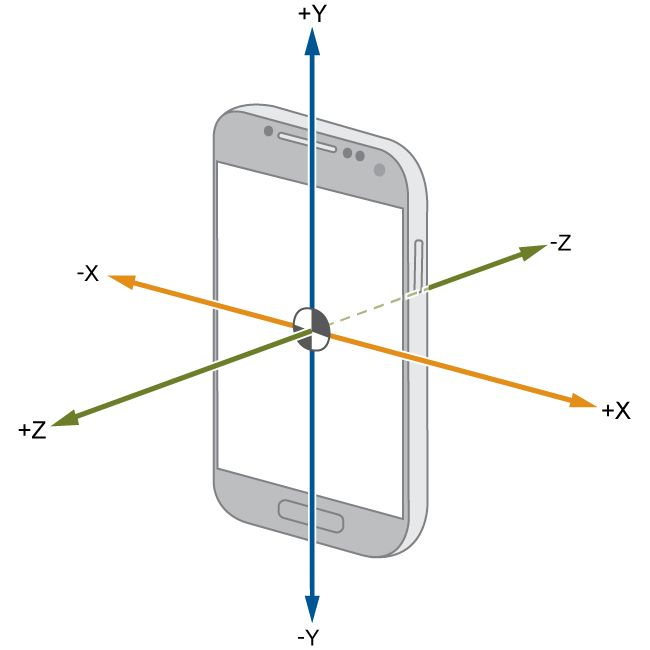
\includegraphics[width=3.0cm]{figures/andereAfb/assenstelsel.JPG}
    \caption{Oriëntataie van de assen}
\end{wrapfigure}


\subsection{Oriëntatie van het toestel}

De oriëntatie van de Z-as hebben we alreeds bepaald door het toestel plat met het scherm naar boven en het scherm naar beneden te leggen. We kunnen nu de oriëntatie van de X-as 

vinden door het toestel met de volumeknop naar boven en naar beneden op de tafel te plaatsen. De oriëntatie van de Y-as vinden we door de gsm recht of omgekeerd op tafel te plaatsen. Zo lezen we af waar deze waarden positief en negatief zijn. De gevonden oriëntatie van de assen wordt afgebeeld in figuur 2.


\section{Ruis}

Wanneer we de metingen - van het toestel in rust - onder de loep nemen, valt op dat we variabiliteit observeren. Er zit dus ruis op de metingen, want we zouden verwachten dat dit niet het geval is. Wanneer we deze waarden plotten - Figuur 3, pagina 2 - wordt deze opmerkelijke bevinding zeer duidelijk; er is altijd een bepaalde hoeveelheid schommeling.

\begin{itemize}
    \item Amplitude: 0.18
    \item Gemiddelde afwijking: 0.02
    \item maximale afwijking: 0.16
\end{itemize}
%\begin{wrapfigure}{ht!}{12.0cm}
    %\label{wrap-fig:3}
    %\includegraphics[width=16.0cm]{GemiddeldeAfw.png}
    %\caption{Grafische voorstelling Z-waarden doorheen de tijd}
%\end{wrapfigure}
\begin{figure}[!h]
    \centering
    \includegraphics[scale=0.65]{figures/andereAfb/GemiddeldeAfw.png}
    \caption{Grafische voorstelling Z-waarden doorheen de tijd}
    \label{wrap-fig:3}
\end{figure}


\section{Verandering van de waarden onder invloed van een hellingsgraad}
\begin{minipage}{.65\textwidth}
  Wanneer we de telefoon met een bepaalde hoek roteren, zal de valversnelling een prominente invloed hebben op de bevonden waarden. De valversnelling langs de X-as is echter 0. De volgende formules zullen gelden voor de Y- en Z-waarden (in m/s²): 

    \[Ay = Atot*sin \alpha\]
    \[Az= Atot*cos \alpha\]

    Als gemeten waarden vinden we (afgerond tot 0.05 veelvoud):
    \begin{itemize}
        \item 30° - gem(X) = 4.7 - gem(Y) = 0.15 - gem(Z) = 8.5
        \item 45° - gem(X) = 6.75 - gem(Y) = 0.1 - gem(Z) = 7.1
        \item 60° - gem(X) = 8.2 - gem(Y) = 0.2 - gem(Z) = 5.2
    \end{itemize}
    Wanneer we de bekomen waarden na invoering vergelijken met de gemeten waarden, zien we dat deze overeenstemmen.
\end{minipage}%
\begin{minipage}{.35\textwidth}
  \centering
  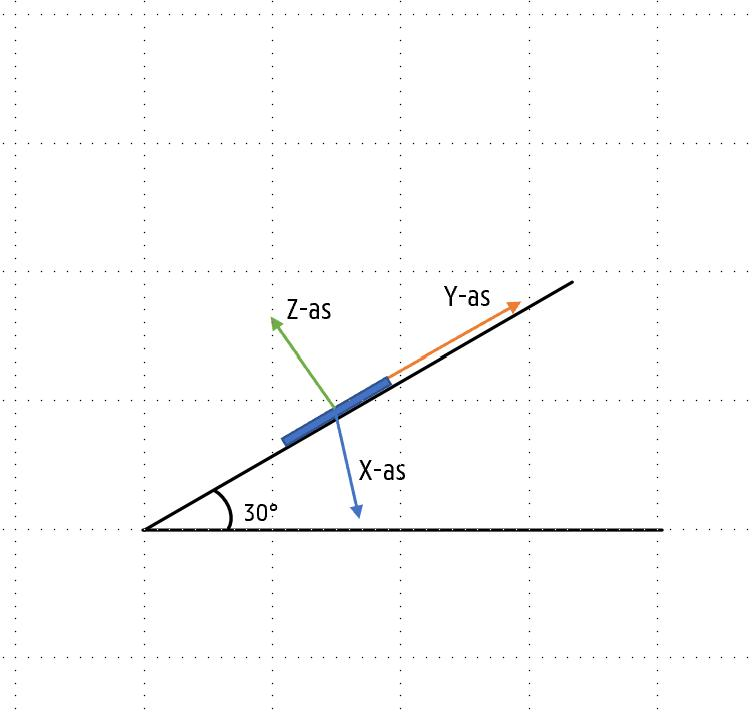
\includegraphics[width=.7\linewidth]{figures/andereAfb/tafb.JPG}
 
  \label{fig:test2}
  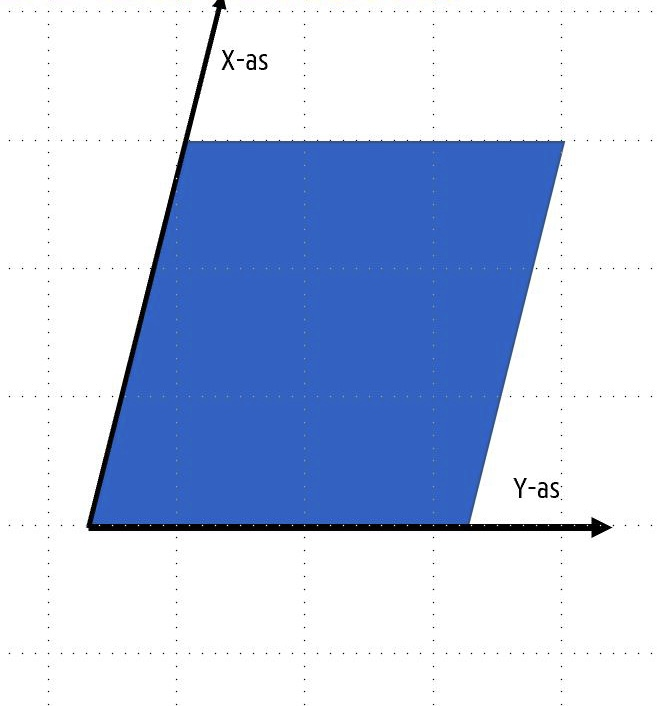
\includegraphics[width=.7\linewidth]{figures/andereAfb/afb.jpg}

\end{minipage}



\section{Denkbeeldig canvas}
\begin{minipage}{.60\textwidth}
  Beschouw als denkbeeldig canvas een vierkant in het XY-vlak. We tekenen het vierkant beginnend uit de linkerhoek.
Wanneer we de eerste zijde tekenen - naar rechts, zal enkel de X-waarde veranderen. Deze zal toenemen in waarde. Wanneer we vervolgens de 2e zijde tekenen, en het toestel naar voren verschuiven, zal enkel de Y-as veranderen in waarde. De waarde van de Y-as zal toenemen. Vervolgens herhalen we wat we net gedaan hebben in de omgekeerde richting en eindigen we waar we gekomen zijn.
\\ Indien we dit met de hand doen, zou er natuurlijk een hoeveelheid ruis zijn. De maximale afwijking van de gemiddelde waarden zou relatief hoog zijn tegenover de waarden die we maten met het toestel in rust. 
\end{minipage}
\begin{minipage}{.40\textwidth}
  \centering
  \caption{Grafische voorstelling van het denkbeeldig canvas}
  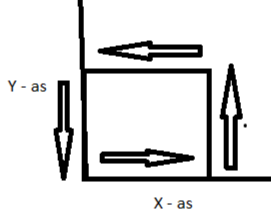
\includegraphics[width=.8\linewidth]{figures/andereAfb/denkbeeldigCanvas.png}
  \label{wrap-fig:5}
\end{minipage}


\end{document}

